\documentclass[12pt, a4paper]{article}
\usepackage{pdfpages}
\usepackage{fancyhdr,amssymb,amsmath,amsthm,bbm,enumerate,mdwlist,url,multirow,hyperref,graphicx}

\usepackage[slovene]{babel}
\usepackage[utf8]{inputenc}
\usepackage[T1]{fontenc}
\graphicspath{ {./images/} }
\pagestyle{plain}

\title{ Finančni praktikum \\\vspace{3cm} {\huge \textbf{Vizing type conjecture for $k$-total rainbow domination number}}\vspace{8mm}}
\author{Avtorja: \\[1.5mm] Brina Pirc, Marcel Špehonja \\ \vspace{6cm}
\\ Univerza v Ljubljani \\[1.5mm]
Fakulteta za matematiko in fiziko \vspace{2cm}}
\date{November, 2019}

\begin{document}

\begin{titlepage}
\clearpage \maketitle
\thispagestyle{empty}
\end{titlepage}

\hypersetup{hidelinks}
\thispagestyle{empty}
\hypersetup{linkcolor = black}
\tableofcontents
\pagebreak


\section{Predstavitev problema}
\subsection{Naloga}
Ukrajinski matematik Vadim G. Vizing je leta 1963 postavil znano domnevo, da je produkt dominantnih števil grafov G in H kvečjemu manjši od dominantnega števila kartezičnega produkta teh dveh grafov. Medtem ko dokaz te domneve še vedno ostaja eden večjih problemov v teoriji grafov, se bova v svojem projektu spraševala, ali lahko pridemo bližje potrditvi (oz. zavrnitvi) naslednje domneve Vizingovega tipa: 

\textbf{Domneva 4}:  Naj bosta $G$ in $H$ povezana, neusmerjena grafa in $k$ $\geq$ $2$. Potem velja: $$\gamma_{krt}(G) \cdot \gamma_{krt}(H) \geq 2 \cdot \gamma_{krt}(G \Box H).$$
Pri tem je $\gamma_{krt}(G)$ oznaka za totalno dominantno število grafa $G$, kartezično pomnoženega s $K$-polnim grafom, torej $\gamma_{krt}(G)$ $=$ $\gamma_{t}(G \Box K_k)$.

\subsection{Definicije}

\underline{\textsc{Dominantna množica}}: dominantna množica grafa $G = (V,E)$ je podmnožica vozlišč $D \subset V$, za katero velja, da ima vsako vozlišče $v$ iz $V \textbackslash D$ vsaj enega soseda, ki je element $D$.
\underline{\textsc{Dominantno število}}: dominantno število grafa $G$ je število vozlišč v najmanjši dominantni množici dominantne množice. \\
\underline{\textsc{Totalno dominantno število}}: je enako dominantnemu številu, z izjemo tega, da morajo imeti elementi v totalni dominantni množici prav tako povezavo z enim iz te množice. Torej prav vsako vozlišče grafa G, brez izjeme, mora imeti soseda v totalni dominantni množici (da je sam del te množice ne zadostuje). \\
\underline{\textsc{Kartezijski produkt}}: grafov $G = (V, E)$ in $H = (V^{\prime}, E^{\prime})$ je graf $G \Box H$ z naborom vozlišč $V \times V^{\prime}$ ter povezavami med $(v, v^{\prime})$ in $(u, u^{\prime})$, če je obstajala povezava med $v$ in $u$ ali med $v^{\prime}$ in $u^{\prime}$. \\
\underline{\textsc{Total $k$-rainbow domination number}}: je totalno dominantno število grafa $G$, kartezijsko pomnoženega z grafom $K_k$, kar je oznaka za $k$-poln graf. \\

\section{Pristop k reševanju}
Za opravljanje projekta sva uporabljala programski jezik $Sage$ na platformi $Cocalc$. Najina naloga je bila poiskati protiprimer domneve Vizingovega tipa, torej poiskati taka grafa $G$ in $H$, kjer neenakost ne velja. Sprva sva definirala funkcijo, ki sprejme dva grafa $G$ in $H$ ter koeficient $k$, vrne pa tako število $c$, za katero velja enakost $\gamma_{krt}(G) \cdot \gamma_{krt}(H) = c \cdot \gamma_{krt}(G \Box H)$. 
\begin{figure}[h!]
\centering
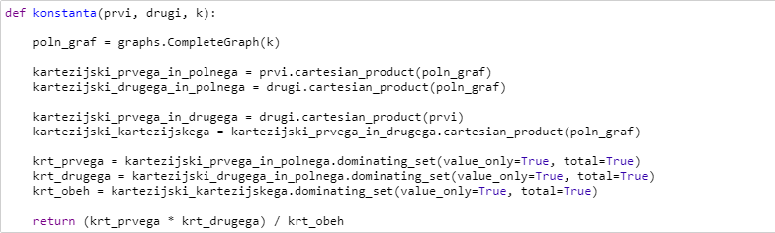
\includegraphics[width=\linewidth]{slika_1}
\end{figure} \\
Če torej dana domneva drži, mora biti $c \leq 2$ za poljuben par povezanih grafov ter podan $k$. Cij projekta je bil poiskati primer, pri katerem bo $c>2$. Seveda je to težek problem, zato sva sprva opazovala, kaj se dogaja pri manjših grafih $G$ in $H$. Postopoma sva povečevala število vozlišč. Pri manjših grafih do 5 vozlišč sva skušala preizkusiti vse možnosti, pri večjih grafih pa sva s pomočjo hevristike dodajala ali odvzemala povezave in sistematično raziskovala izide. Tu sva uporabila metodo $simulated$ $annealing$. Hkrati sva počasi povečevala tudi $k$. Posebej sva obravnavala tudi dvodelne grafe, poti in drevesa ter ugotavljala kako se obnašajo v dani neenakosti. Zanimalo naju je predvsem pri katerem paru grafov je $c$ največji, če je $k$ konstanten.

\section{Testiranje}
\subsection{Vsi grafi do 5 vozlišč}
Najprej sva generirala vse povezane grafe od 2 do 5 vozlišč, ki jih je 30. Nato sva vzela vse možne kombinacije parov teh grafov, torej $\binom{31}{2}=465$, ter vse te kombinacije vstavila v najino funkcijo, ki vrne iskan koeficient $c$. Dane rezultate sva nato vstavila v novi funkciji, ki sta poiskali maksimum in minimum izračunanih $c$-jev, ter izpisali pare grafov pri katerih je prišlo do teh ekstremov. \\
Pri prvem poskusu je bil $k=2$: Maximum iskanih koeficientov $c$ je bil enak 2, število parov pri katerih je prišlo do maksimuma pa je bilo kar 10. Torej je pri desetih različnih parih grafov prišlo do enakosti domneve $\gamma_{krt}(G) \cdot \gamma_{krt}(H) = 2 \cdot \gamma_{krt}(G \Box H)$. Minimum koeficienta $c$ je bil 2/5. \\
$k=3$:  Maximum $c$-ja je bil sedaj 5/3, kar je manj od 2, število parov pri katerih je prišlo do maksimuma pa 6. To nakazuje na domnevo da, ko povečujemo število $k$ se koeficient $c$ manjša. Minimum koeficienta $c$ je bil 9/13. \\
$k=4$: Maximum $c$-ja se je ponovno zmanjšal pri $k=4$ , saj je 20/13, kar je manj od 5/3. Minimum koeficienta $c$ pa je 1.
Zaenkrat bi lahko sklepali, da ko povečujemo $k$, se maximum koeficienta $c$ manjša, minimum pa veča. Da bi to potrdili moramo testirati še grafe z več vozlišči. \\

\subsection{Dvodelni grafi}
Podobno, kot pri prejšnjem primeru sva generirala grafe, tokrat dvodelne povezane do 6 vozlišč. Teh je 27, torej vseh možnih kombinacij parov je $\binom{28}{2}=378$. Tudi ta primer potrdi naše sklepanje, da se maksimum $c$-ja zmanjša, minimum pa poveča, ob večanju $k$-ja, saj smo pri $k=2$ dobili max(c)=2, min(c)=1/3, pri $k=3$ smo dobili max(c)=5/3, min(c)=9/16, pri $k=4$ pa max(c)=30/19, min(c)=4/5. \\
Vidimo pri maksimum velja : $2>5/3>30/19$, se manjša, \\
pri minimum pa: $1/3<9/16<4/5$, se veča. \\
Tudi število parov, ki dosežejo maksimum se zmanjša, saj je pri $k=2$ maksimum doseglo 15 različnih parov, pri $k=3$, 10 različnih, pri $k=4$ pa le 2 različna para. \\
Vzela sva tudi dvodelne grafe do 7 vozlišč (71 možnih), kjer sva pri generiranju parov odvzela tiste, ki so bili že obravnavani v prejšnjem primeru (kombinacij je torej $\binom{72}{2} - 378=2178$). Dobili smo sledeče: \\
$k=2$:  max(c) = 2 , min(c) = 2/7 \\
$k=3$:  max(c)= 12/7,  min(c)=9/19 \\
Ponovno rezultati potrjujejo našo domnevo.

\subsection{Poti}
Sprva sva opazovala vse kartezijske produkte poti na $i$ vozliščih (kar je znašalo $i\cdot(i+1)/2$ rezultatov). Ugotovila pa sva, da se večinoma večje vrednosti za $c$ nahajajo na začetku, torej da z večanjem vozlišč $c$ v povprečju pada. S povečevanjem vozlišč bi tako dobivali le enake maksimume za $c$, saj se ti pojavijo pri manjših grafih. Zato sva se odločila, da z vsakim naslednjim poskusom zajameva le grafe, ki jih prej še nisva. Torej, da fiksiramo $j$ (1. graf je torej $P_j$) in opazujemo obnašanje $c$-ja, ko število vozlišč 2.grafa teče od 2 do $j$ (GLEJ KODO). Dobila sva zanimive rezultate, predvsem je zanimiv pojav pri grafu $P_4$. Kadar je $k=2$, se največji $c$ vedno pojavi v kombinaciji s slednjim grafom. Prišli smo do največ poti na 12 vozliščih, za izračun $c$-ja pri podanih $P_9$ in $P_{12}$ je program potreboval več kot en dan, nato se je ustavil (ne da bi vrnil vrednost). Kljub temu bi lahko iz vzorca sklepali, da je največji $c$ dosežen pri $P_4$ in $P_{12}$. Pri $k=2$ je maksimalni $c=2$, dobimo pa ga z grafoma 4-poti. Za $k=3$ sva najdlje prišla na 9-poti, pa še to brez 8,8-poti, 7,9-poti, 8,9-poti in 9,9-poti. Največji $c$ pri dobljenih rezultatih je znašal 20/13 (za 4,5-poti). Pri $k=4$ je $c$ največji z grafoma 6,6-poti, in sicer $c=4/3$ (do 6 vozlišč). \\
Ugotovila sva, da če so $n$, $m$ in $k$ dovolj veliki, bo zgoraj na ulomku $n \cdot m$, saj bo naše $k$-totalno dominantno število pri $k \geq 4$ enako številu vozlišč poti. To velja za vsaj 2-pot. Tudi pri 3-polnem grafu dobimo vzorec, vendar ne tako jasen: $[2,2,$ $3,4,5,6,$ $6,7,8,9,10,$ $10,11,12,13,14,$ $14, ...]$, torej bo zmnožek $3-rt$ števil grafov $n$ in $m$ poti v primerjavi s $k \geq 4$ padal, ko sta $n$ in $m$ vedno večja (v smislu da je pri $n=7$ in $m=3$ v prvem primeru $3 \cdot 7=21$, pri $k=3$ pa $3 \cdot 6=18$). Pri $k=2$ pa je $2-rt$ število enako $[2,2,2,$ $4,4,4,$ $6,6,6,$ $...]$, kjer je indeks v seznamu enak številu vozlišč poti (prvi element ima indeks 1). Tu je zmnožek še manjši (za $n=7$, $m=3$ dobimo $2 \cdot 6=12$). To je tudi smiselno, saj večji kot je graf, večje število vozlišč bo v dominantni množici. Pri dotičnem primeru, torej 3-poti, 7-poti in $k$ iz (2, 3, 4), $c$ z naraščanjem $k$ pada.\\
Problem, s katerim sva se soočala vseskozi projekt, je bil zahtevnost računanja $k$-totalnih dominantnih števil. Za manjše grafe in manjše $k$, kar je pri poteh pomenilo do 10 vozlišč, sva si pri računanju »grafa« (kot se je imenovala funkcija, ki je vračala najin $c$). Za $k=3$ je bilo že 9 vozlišč na meji zmogljivosti, saj je program po 7 urah računanja vrnil največ (7,8) in (6,9), torej ne pa kaj se zgodi, če opazujemo $8\times8$, $7\times9$, $8\times9$ in $9\times9$ poti. \\

\subsection{Drevesa}
Najprej sva naredila seznam neizomorfnih dreves. Takšnih dreves na do 10 vozliščih je 201. Ker so bile že pri poteh na 12 vozliščih in $k=2$ težave, sva tu pričakovala še počasnejše računanje. Pri $k=2$ je bil največji $c=2$. Skušala sva računati le za drevesa na 9 vozliščih, vendar jih je izračunal zelo malo, največ $T[48]$, $T[201]$. Pri $k=3$ je izračunal največ drevesa na do 7 vozlišč, $c=35/22$; pri $k=4$ je $c=4/3$ (vozlišča do 5); $k=5$, $c=5/4$ (do 5 vozlišč). \\
\pagebreak

\subsection{Simulated annealing}
Za večje grafe sva definirala psevdokodo po metodi simulated annealing:
\begin{figure}[h!]
\centering
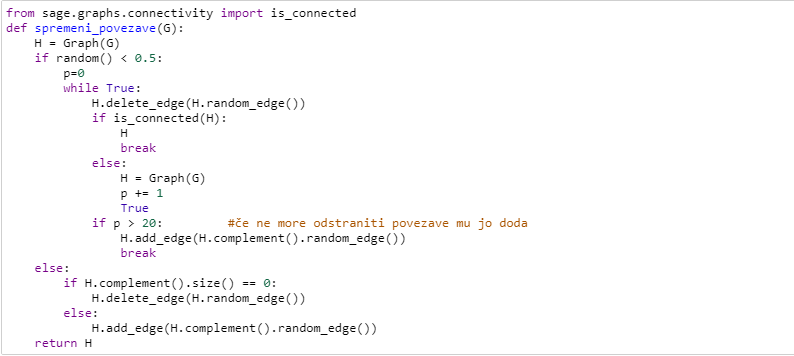
\includegraphics[width=13.5cm]{slika_2}
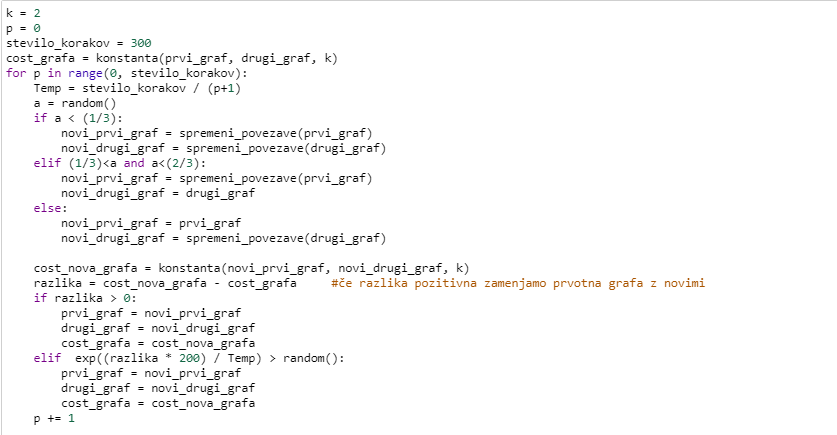
\includegraphics[width=13.5cm]{slika_3}
\end{figure} \\
Ta algoritem sprejme dva naključna grafa na določenem številu vozlišč, ki jima nato spreminja povezave, s funkcijo $spremeni_povezave()$ in ugotavlja kako morata bti ta dva grafa povezana, da dosežemo čim večji koeficient $c$. Tu sva vstavljala grafe velikosti od 8 do 10 vozlišč. Prav vsi poskusi so ponovno pokazali, da ko povečamo $k$ se koeficient $c$ zmanjša. Pri $k=2$ algoritem večinoma vrne vrednost $c=2$. Takoj ko $k$ povečamo pa vrednost $c$-ja pade. V vseh najinih poskusih pa vrednost koeficienta $c$ nikoli ni bila večja od 2. To pomeni, da nisva našla protiprimera obravnavane domneve Vizingovega tipa.



\end{document}




